% Ensalada sunomono
\newpage
\begin{recipe}[source={Adaptación propia},
portion={2-4 porciones},
preparationtime={\unit[20]{Minutos}}
]{Ensalada Sunomono}
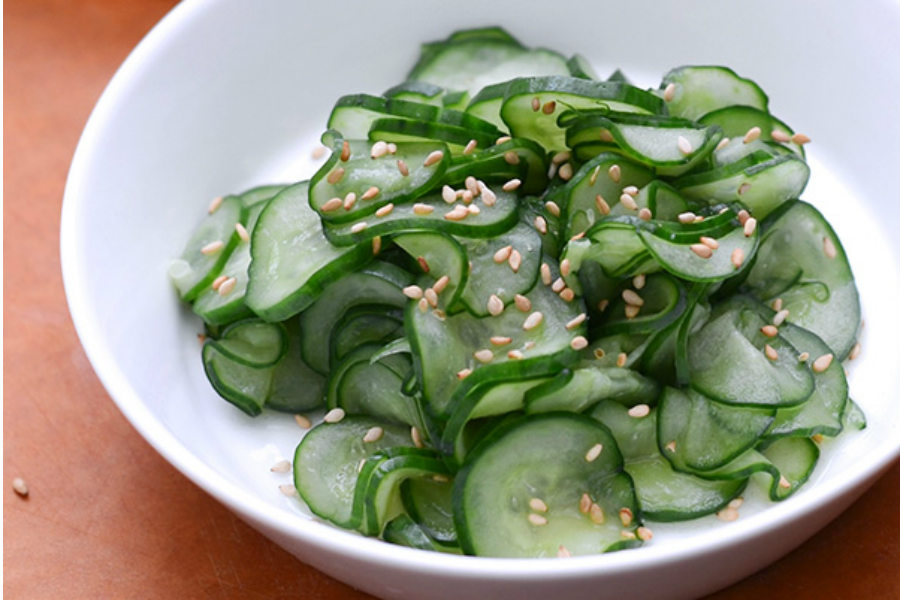
\includegraphics[width=0.25\textwidth]{sunomono}
\introduction{
Una receta que pillé en algún video de youtube. Me gustó su simplesa y lo rico que es
}
\ingredients{
    2 & pepinos \\
    1/2 & cucharada de sésamo \\
    1 & cucharadita de sal \\
    4 & cucharadas de vinagre de arroz \\
    1/2 & cucharada de salsa de soja \\
    2 & cucharadas de azúcar 
}
\preparation{
    \begin{enumerate}
        \item Cortar en láminas delgadas los pepinos y lavar con agua con sal unos 10 minutos.
        \item Escurrir el agua y comenzar a aliñar, integrando los demás ingredientes.
        \item Una vez revuelto, reservar en el refrigador al menos una media hora antes de servir.
    \end{enumerate}
}
\end{recipe}